\chapter{Background}
This chapter gives an overview of the necessary background information required for this research. Air quality monitors are explained in a general way with its use, capabilities and sensors. Passive network eavesdropping and private information inference are introduced as this will be the vulnerability exploit in this research. Lastly, this chapter gives an overview of the communication protocol IEEE 802.11, Wi-Fi, as the air quality monitors used in this research communicates over it and the sniffing will take place on this protocol.

\section{Air Quality Monitors}
Air quality monitors are used as sensors to collect sensor data from different sources in the air \cite{GeneralAirQualityMonitor}. The IoT devices can store data in different ways. Cloud storing is the most preferred storage solution for IoT devices, but also local servers, internal storage and SD cards can be used to store data from IoT devices and air quality monitors \cite{AQMBigSource}. Displaying data to users of air quality monitors is an important factor to give the user either information about the indoor air quality, or recommendations on how to better the air \cite{AQMBigSource}. The most developed and recent method of doing so, is through an app on the users mobile phone, but also solutions where users can login to a web-site exists. Many air quality monitors also have the functionality of a screen on the device that shows certain values from the sensors. Some of these can also be interactive \cite{AQMBigSource}.
\\\\
As indoor air quality monitors can be equipped with different features, a brief explanation of some of the sensors an air quality monitor can be equipped with is necessary to understand why and how private information can be gathered from these sensors:
\begin{itemize}
    \item \(CO_2\)\\
        Carbon Dioxide, \(CO_2\), is a chemical formula that is made by human or animal combustion, in addition to other larger combustion processes \cite{CO2}. This implicates that the more humans or animals that are in the same indoor environment as the air quality monitor, the higher occurrence of \(CO_2\) will be collected by the sensor and transmitted to the air quality monitors receiver. However, plants and sunlight can bind \(CO_2\) and reduce the amount of \(CO_2\) particles in an indoor environment. Also bad or irregular ventilation will make the \(CO_2\) levels grow. \\
    \item Radon\\
        Radon is a radioactive gas that is strongly recommended to be measured in Norwegian indoor environments \cite{Radon}. The gas does not smell, is invisible and is carcinogenic which makes it an attractive feature to include on the air quality monitor. Radon evaporates from the ground and into air and is therefore not made by human actions in an indoor environment.\\
    \item Noise\\
        Noise is an interesting feature of some air quality monitors as it is considered a health problem \cite{Noise}. Exposure to loud noises at a small amount of time or long-term noise can harm peoples health. Especially when considering a work environment where workers need to concentrate, noises over long periods of time can result in hearing difficulties or problems communicating. As many work from home and we use a lot of time in our home, the problem is also applicable here. \\
    \item VOC\\
        Volatile organic compounds, VOC, is a collective term for any combination of carbon, with the exception of carbon monoxide, carbon dioxide, carbonic acid, metallic carbides or carbonates and ammonium carbonate \cite{VOC}. These harmful compounds can be found in gases from building materials or smoking, cleaning articles, painting or cooking to mention some. TVOC is a term for defining the total amount of VOCs. The amount of VOC in the indoor environment can be simply reduced by ensuring fresh air and using kitchen fans to prevent the articles from circulating the indoor air to be breathed by users \cite{RecommendedIAQ}.\\
     \item HCHO\\
        HCHO is the chemical formula for formaldehyde which is a gas that can cause severe health effects, like headache and irritation of airways \cite{HCHO}. The gas contains a strong odor and is flammable when it has room temperature, but is colorless. People can be exposed to HCHO from several different sources such as manufacture wood products, building materials, fertilizers, cigarettes, paint, glue or even medicines and cosmetics. Formaldehyde is classified as a VOC.\\
    \item Humidity\\
        Humidity is calculated from the ratio between water vapor in the air compared to the maximum amount of water vapor possible in the air if the air was saturated \cite{RecommendedIAQ}. Even tough humans can endure high variations in humidity, very low percentages of humidity can result in health problems such as irritated eyes, dry skin or dry moucus membranes. While high humidity can begin mold processes that can damage indoor furniture or walls and lead to health problems like asthma or allergy if evolved. The humidity is correlated by temperature, which means that variations in temperature can effect the humidity percentage. Normal user behaviour that can affect the humidity is taking a shower, drying clothes or cooking. \\
    \item Temperature\\
        Temperature is a measure unit for how hot or cold the environment is and is measured using a thermometer. Temperature is the most commonly used unit for how comfortable humans feel. Temperature can affect humans health on both ends of the scale. A too high temperature can result in lack of energy and sleepiness and a too low temperature can result in reduced muscle function or heighten symptoms of rheumatism \cite{Temp}.\\
\end{itemize}

Several factors plays a key part when selecting which air quality monitor most suitable for the users needs. Even tough many devices are pre-calibrated when available in store, a test on the specific environment should be done. Considering the different functionality an air quality monitor can have, it is also important to look into transmission range, power consumption and requirements for maintenance \cite{AQMBigSource}. However, the main goal of an air quality monitor is to monitor the air and therefore looking into which kind of sensors the devices have should be a top priority when selecting your device. Air quality monitors can specialize in one measuring unit in the air or have the functionality to measure several air quality factors, such as \(CO_2\), radon, HCHO, noise, VOC, humidity or temperature. The air quality monitors are incorporated in users homes and therefore the appearance of the device will also be a considerable factor for choosing the right device, but can again be affected by the price of the device \cite{IAQMonitorCommunicationReview}. 
\\\\
There are several companies that manufacture and sell air quality monitors. Some companies sell air quality monitors who's main goal is to monitor the air and report to the user and are more specialized in air quality monitor as an IoT device, such as Airthings \cite{Airthings}, Netatmo \cite{Netatmo} and Mill \cite{Mill}. While other companies integrates the air quality monitor with another device that has a main goal of changing humidity or \(CO_2\) levels in the indoor environment based on the sensor values to better the indoor air conditions. Examples of these are Phillips \cite{Philips} and Dyson \cite{Dyson}. These companies have different air quality monitors that users can choose from based on their needs. But they emphasises what kind of air quality contaminant their devices are able to monitor. 
\\\\

\subsection{Private Information Inference}
Considering the amount of information an air quality monitor can collect about an individual or a smart home, privacy leakage is a vulnerability \cite{SecPrivSmartCity}. Privacy is referred to as every persons right to have control over their own data, hereby knowing how their data is used or distributed to other parties \cite{IoTSecPrivSafeEth}. When malicious attackers tries to gather sensitive information about an individual user or group of users, a privacy attack is carried out \cite{CyberEntitySecInIoT}. The aim of the attacker is then to target the confidentiality of the user, while gathering information such as location, preferences, personal behaviour or similar private information. A challenge with an IoT system compared to other computer systems is that the IoT devices are always on, connected in a users home and sense the user behaviour in a passive and non-intrusive way. This makes it even more difficult to understand the scope of all the private information gathered by an IoT system \cite{IoTSecPrivSafeEth}.
\\\\
IoT systems in a smart home is often made up by different brands and communication protocol and does not follow a standard like IoT systems in an industrial environment can \cite{IoTPrivSecSmarthome}. There is no central management of doing security patches or having a strong baseline of security that protects the privacy a sensor holds. A big threat to IoT privacy is identification and profiling, where an attacker can link a user to their behaviour in the IoT environment \cite{IoTSecPrivSafeEth}. An attacker can then study the data from a users environment and identify what that user is doing. An example can be that by reading an increase in data from an IoT device communicating to a server for IoT coffee appliances, an attacker can know that the users is making coffee at a specific time a day, and by collecting this data over a longer period of time, knowing the routines of a user. Even tough a morning coffee can be something a user posts openly on social medias, not having control of their data and who can access and process it is a violation of privacy. This could also be launched against many IoT devices in an environment at once and even correlating when a user is home and not and use this to commit physical attacks, like burglary for example. 
\\\\
A challenge when it comes to privacy for IoT systems is weighting functionality against privacy and security \cite{PrivacyIoTSurvey}. There are security measures that can be implemented for the devices to mitigate private information inference, such as authentication and authorization, data anonymization and cryptology. However, not only attackers wanting to know about users private information poses a threat to users IoT data, but also interested parties wanting to know user behaviour to make more suitable solutions and targeted advertisement to earn more money. So users needs to be aware of where their data are shared to ensure that private information is not shared without their knowledge. On the other side, users are requesting better functionality for the IoT devices, wanting them to behave more customized and optimized to their needs which requires more data to be shared. Although security vs privacy is a known issue in the computer world, IoT devices are resource restrained and preferably as ascetically integrated in users home as possible, and therefore applying security measures to ensure privacy is a challenge for these devices \cite{PrivacyIoTSurvey}. 

\subsection{Passive Network Eavesdropping}
Eavesdropping network communication can either be passive or active. When an attacker conducts an active eavesdropping attack on a target, the data in the communication link is both inferred and modified \cite{Eavesdropping}. While in a passive network eavesdropping attack, the eavesdropper does not modify any data on the link, but simply aims to gather data transmitted without changing the communication. The overall goal of eavesdropping is therefore often to access private information that are being sent on the channel. This can be anything from credentials to secret messages, or as in this research, private information about users and their habits \cite{Eavesdropping}. Since the communication is not effected by a passive network eavesdropping attack, the attacker does not need to be as careful in disguising itself as in an active attack.  
\\\\
There are security measures to implement to reduce the chance of being eavesdropped, both actively and passively. Since an eavesdroppers goal is to listen in on the communication, encrypting the traffic is an effective way to make it harder to conduct an eavesdropping attack. Also, covert channels that hide the identity of the communicating parties can be used to prevent the eavesdropper from finding the right communication channel to eavesdrop \cite{Eavesdropping}.
\\\\
To perform a passive network eavesdropping attack on wireless communication channels, it is not necessary to be able to join the targeted network, but the attacker needs to be within signal range of the network \cite{WifiEavesdropEnc}. To be able to carry out a passive network eavesdropping attack, the right hardware and software must be configured \cite{Sniffingtech}. A wireless network sniffer can collect wireless traffic for the corresponding communication protocol within its signal range. To be able to use a wireless sniffer to carry out a passive network eavesdropping attack, this device needs to be configured to capture packets that are not meant for the device it is connected to, normally a computer or server, but every packet within its signal strength. This is often called promiscuous or monitor mode. It exists a number of network sniffers for every wireless communication protocol, such as Wi-Fi, Bluetooth, ZigBee or Z-wave to mention some \cite{Sniffingtech}. Some computers even have a built in network card that can be used to monitor traffic, not directed to itself, on a wireless network. Once the sniffer is configured to capture packets, a monitoring tool is necessary to collect, store and analyze the packets. Such as for the sniffers, there are a lot of different software monitoring tools that can be used for this purpose and it is often recommended to use specific ones based on the operating system the server or computer that are carrying out the attack uses. However, a very common choice for both Linux and Windows is Wireshark \cite{Wireshark}, which is a free online-available monitoring tool. When both the hardware sniffer and software monitoring tool are configured correctly the network eavesdropping attack can be carried out. 

\section{Communication Protocols}
Air Quality Monitors send their sensor data to remote server for storing and analyzing of the data and communicates with a hub or a users phone to display the values of the different air contaminants. As they exists with different functionality and specifications, their communication protocols differs, like other groups of IoT devices \cite{AQMBigSource}. Wi-Fi is the most preferred protocol with Bluetooth and ZigBee following \cite{saini2020indoor}. As this thesis is delimited to air quality monitor devices using Wi-Fi to communicate, the next subsection will elaborate on this protocol and specifications to be used further in this thesis through testing and analysis. 

\subsection{IEEE 802.11 - Wi-Fi}
Wireless Fidelity (Wi-Fi) \cite{WiFiAlliance} is one of the worlds most used technology for communicating and is defined, developed and standardized by WiFi Alliance \cite{WiFiAlliance}. Wi-Fi is based on the standard IEEE 802.11 Wireless LAN set by IEEE Standard for Information Technology \cite{WifiStandard}. The transmission range for Wi-Fi is up to 100 meters and it uses 5-60GHz in the frequency band \cite{IAQMonitorCommunicationReview}.
\\\\
In a Wi-Fi Local Area Network (LAN) each communicating node, such as computers, IoT devices or mobile phones, connects to an Access Point (AP), which connects the devices to the Internet \cite{Datacom}. The AP works as a base station of the devices and these units makes up the fundamental for Wi-Fi, called Basic Service Set (BSS). The AP connects to the Internet commonly using a switch or router, which can be integrated in the same physical device. When connecting to a Wi-Fi network, an identifier, often set as a default name by the Internet Service Provider (ISP) or a customized name made by the administrator of the network, is visible for devices trying to connect the network. This identifier is called a Service Set Identifier (SSID) and is used to distinguish multiple APs to choose the right one to connect to. Each AP will periodically send out broadcast messages in a beacon frame containing their MAC address and SSID. When the device has chosen the right AP to connect to based on the beacon frame, an association begins between the AP and the device to create a wireless link between the two. This link will be used by both the AP, to send packets from the Internet directed to the device and from the device to Internet, and by the device, to receive and send packets to the Internet \cite{Datacom}. 
\\\\
A network packet sent from a device communicating in a Wi-Fi network is called a data frame \cite{Datacom}. The data frame is illustrated in figure \ref{fig:WiFiDataframe}.

\begin{figure}
    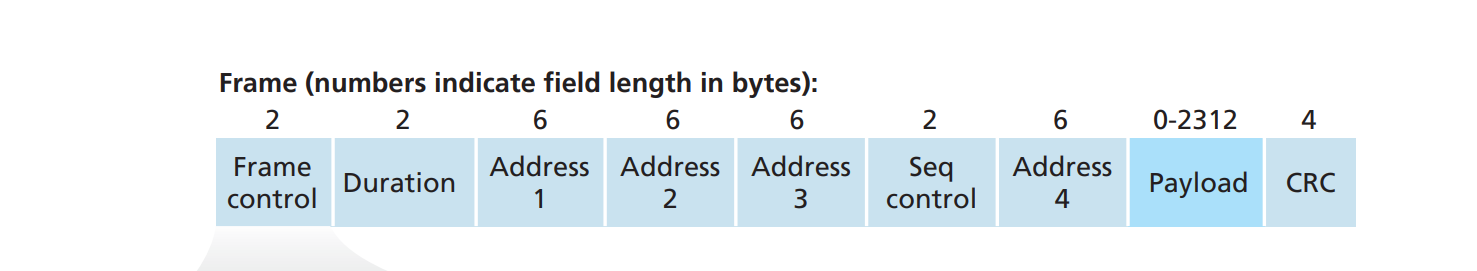
\includegraphics[width=1\textwidth]{figures/WifiDataFrame.png}
    \caption{Wi-Fi Data Frame \cite{Datacom}}
    \centering
    \label{fig:WiFiDataframe}
\end{figure}

The frame control field contains several different fields for encryption, acknowledgment and the association to mention some \cite{Datacom}. The duration field holds the value of how long a to reserve a channel to transmit the data frame and acknowledgement. Sequence numbers are used for a receiver to be able to make up the order of which the packets are sent if they arrive in the wrong order over the medium. As shown in the figure \ref{fig:WiFiDataframe}, there are 4 different MAC address fields. Address 1 contains the MAC address to the destination of the packet and address 2 contains the MAC address for the source of the packet. Address 3 contains the MAC address of the router connected to the BSS and address 4 contains the MAC address for XXXXX. The Cyclic-Redundancy Check (CRC) field is controlled by the receiver to check for bit errors. The final field is the payload where the transmitted data relies in an IP or ARP packet. 
\\\\
Understanding different packets in a Wi-Fi network
ACK
    Data
    QoS
    Authentication
\\\\
Traffic patterns of IoT devices communicating on Wifi
    Association
    User behaviour
    Updates
\\\\
Wifi security - network eavesdropping and privacy.